\documentclass[11pt,a4paper]{scrbook}
\usepackage[utf8]{inputenc}
\usepackage[T1]{fontenc}
\usepackage[pdftex]{graphicx}
\usepackage[ngerman, english]{babel} % the language specified at the end of the list will be used !!
\usepackage{colortbl}	
\usepackage{xcolor}
\usepackage{soul}
\usepackage{comment}
\usepackage{etoolbox}
\usepackage{geometry}
% \usepackage[landscape]{geometry}
\usepackage{tikz}
\usetikzlibrary{timeline}
\usepackage{lscape}
% For APA referencing style
\usepackage[natbibapa]{apacite}
\bibliographystyle{apacite}
% For the positioning of the image
\usepackage{float}
\usepackage[ddmmyyyy]{datetime}
\usepackage{changepage}   % for the adjustwidth environment
\usepackage[acronym,nomain]{glossaries}

 
%%%%%%%%%%%%%%%%%%%%%%%%%%%%%%%%%%%%%%%%%%%%%%%%%%
 
\newacronym{ER}{ER}{Emotion Recognition}
\newacronym{SER}{SER}{Speech Emotion Recognition}
\newacronym{EEG}{EEG}{Electroencephalography}
\newacronym{MVP}{MVP}{Minimum Viable Product}
\newacronym{ML}{ML}{Machine Learning}
\newacronym{MTCNN}{MTCNN}{Multi-task Cascaded Convolutional Neural Networks}
\newacronym{AAM}{AAM}{Active Appearance Model}
 
%%%%%%%%%%%%%%%%%%%%%%%%%%%%%%%%%%%%%%%%%%%%%%%%%%%
 


\renewcommand{\familydefault}{\sfdefault}
\definecolor{uhhred}{cmyk}{0,100,100,0}

% following three lines used to get rid of the new pager after each chapter
\makeatletter
\patchcmd{\scr@startchapter}{\if@openright\cleardoublepage\else\clearpage\fi}{}{}{}
\makeatother


\begin{document}
\frontmatter
\newgeometry{centering,left=2cm,right=2cm,top=2cm,bottom=2cm}
\begin{titlepage}

\includegraphics[scale=0.3]{UHH-Logo_2010_Farbe_CMYK.pdf}
\vspace*{1cm}
\Large
\begin{center}
{\color{uhhred}\textbf{\so{EXPOS\'E}}}
\vspace*{1.0cm}\\
{\textbf{for a master's thesis at the University of Hamburg in the Department of Computer Science in the master's programme IT Management and Consulting}}
\vspace*{2.0cm}\\
{\LARGE \textbf{Title:}}
\vspace*{0.4cm}\\
{\LARGE Visual Emotion Recognition In-The-Wild}
%{\LARGE Visual Emotion Recognition In-The-Wild: Prediction of valence/arousal and assessment of application in real-time video consultations }
%{\LARGE Identifying customer intentions in real-time video consultations through emotion recognition: Analysis of viability and value co-creation by implementation of a prototype}
\vspace*{1.5cm}\\
presented by
\vspace*{0.4cm}\\
Tobias Kick
\end{center}
\vspace*{2.5cm}

\noindent
MIN-Faculty \vspace*{0.25cm} \\
Department of Computer Science\vspace*{0.25cm} \\
Research group: Computer Vision\vspace*{0.25cm} \\
Program: IT Management and Consulting\vspace*{0.25cm} \\
Matriculation number: 7213712 \vspace*{0.5cm} \\
%Ggf. Abgabedatum: XX.XX.20XX \vspace*{0.5cm} \\  %TODO Optional, entweder "Ggf. " oder ganze Zeile löschen
Supervisor: Noha Sarhan \vspace*{0.25cm} \\
First assessor: Prof. Dr. Simone Frintrop \vspace*{0.25cm} \\
Second assessor: Dr. Mikko Lauri

\end{titlepage}

\restoregeometry

\tableofcontents

\mainmatter
\setlength{\parindent}{1cm}

%%%%%%%%%%%%%%%%%%%%%%%%%%%%%%%%%%%%%%%%%%%%%%%%%%%%%%%

\chapter{Problem and topic definition}
\begin{comment}
Hier sollten Sie kurz und präzise ihr Thema beschreiben und in den wissenschaftlichen Kontext einordnen. 
Geben Sie auch die aktuelle Relevanz des Themas wieder. 
Machen Sie zudem deutlich, warum Sie sich persönlich für das Thema entschieden haben, aber auch welchen Mehrwert die Wissenschaft und/oder Praxis von der Erörterung dieses Themas hat.

Mögliche Fragestellungen:
•	In welchem Umfeld/Unternehmen wird die Masterarbeit geschrieben?
•	Welche Themen (mit Bezug zur Masterarbeit) stellt das betrachtete Um-feld/Unternehmen vor Herausforderungen? Was ist der Untersuchungsanlass?
•	Was ist das für die Masterarbeit relevante Thema/Objekt, dass diese Herausforderung adressiert?
\end{comment}

The master thesis will be written in cooperation with PPI AG, a Hamburg-based software and consulting firm with focus on the banking and insurance industry. According to IBM, the industry is under immense pressure from new technology, as it is tearing down entry barriers into the market and is opening doors for new financial service providers, like FinTechs.
\citep{IBM:2020:TheImpactOfDigitization} This means, that
\begin{quote}
Competition from startups, internet giants, and industries outside of banking, along with increased regulations, are forcing banks to accelerate their Digital Reinvention. \citep{IBM:2020:TheImpactOfDigitization}
\end{quote}
\vspace{0.1cm}
Herein lies a big opportunity for PPI, who is constantly striving to enable banks and insurances in propelling their Digital Reinvention. This also requires PPI to come up with innovative solutions for their customers, solutions that differentiate them from their competitors and deliver value to the end-customer.
\newline\newline
Therefore, PPI AG is constantly striving to explore and utilize technological advances in order to generate new business opportunities. Thus, this Master thesis's aim is to validate technological advances in the field of Emotion Recognition, more specifically in video call consultations, in order to assist consultants and customers. The goal is to create a prototype which firstly, proves the viability of inferring human intentions from recognized emotions during video calls and secondly, proves that this approach generates added value for PPI AG and their customers.
\newline\newline
Even though it is possible to recognize emotions from facial expressions, speech patterns, and other input signals, this prototype will primarily focus on the recognition of emotions from facial expressions.

%%%%%%%%%%%%%%%%%%%%%%%%%%%%%%%%%%%%%%%%%%%%%%%%%%%%%%%

\chapter{State of research}
\begin{comment}
Wie sieht der aktuelle Forschungsstand zu Ihrem gewählten Thema aus? Hier geben Sie relevante Forschungsergebnisse und aktuelle Studien an, die Sie auf Basis Ihrer beginnenden Sichtung der Literatur recherchieren konnten. Zeigen Sie hier die Forschungslücke und den Beitrag zur Forschung und Praxis auf.

Mögliche Fragestellungen:
•	Warum ist das identifizierte Thema relevant für die Praxis?
•	Warum ist das identifizierte Thema relevant für die Forschung? Besteht hier eine Forschungslücke, dass nicht auf bestehende Konzepte zurückgegriffen werden kann?
•	Wo liegen die Defizite/Herausforderungen/Probleme in dem identifizierten Themengebiet?
\end{comment}

As of today, \gls{ER} systems, unlike \gls{SER} systems \citep{Akcay:2020:SpeechEmotionRecognition(SER)}, are not prevalent in the technology we use on a daily basis, as there are still multiple obstacles that need to be solved. These comprise, for example, available and meaningful training data, as well as better performing algorithms. However, there have been many advances in the last years, which will be summarized as follows: 
\newline\newline
\citet{Salah:2018:Video-BasedEmotionRec} were able to construct a system which can correctly classify emotions expressed in videos. They made use of a discrete emotion model, previosuly proposed by \citeauthor{Briesemeister:2011:DiscreteEmotion} in \citeyear{Briesemeister:2011:DiscreteEmotion}, which allowed them to classify emotions into 7 different emotion classes. 
\newline\newline
This classification approach is still widely used in \gls{ER} research today, next to another approach called Continuous Affective Space. In 2010, the authors \citet{Hupont:2010:FacialEmotionsIn2DAffectiveSpace} came up with a way of measuring emotions as a psychological 2-dimensional continuous affective space. Through mapping emotions into a 2D space they are able to consider intermediate emotional states. In practice, this means, that instead of categorizing emotions, like 'happy' and 'angry', emotions are represented by two variables in a 2-dimensional space.
\newline\newline
The trend in research on \gls{ER} during the last years was strongly defined by the challenge of fusing multiple input signals for better prediction results. Most scientific contributions in this area, like the papers by \citet{Yan:2016:MultiClueFusion} and \citet{Hossain:2019:AudioVisualER}, were fusing audio with visual signals in order to improve their \gls{ER}. Another paper by \citet{Xing:2019:EEGAudioVisual} made use of combining EEG with audio and visual signals. However, the possibilities are not restricted to those mentioned input signals. As the authors \citet{Akcay:2020:SpeechEmotionRecognition(SER)} in a summary on Speech Emotion Recognition (SER) point out, audio signals could be combined with visual signals, physiological signals, linguistic features, mouse movements and keystroke dynamics.
\newline\newline
Current literature about the identification of human intentions through Emotion Recognition is very sparse. The research done in this area is mostly about detecting customer satisfaction. The authors \citet{Kamaruddin:2016:MeasuringCustomerSatisfaction} in their paper "Measuring Customer Satisfaction through Speech using Valence-Arousal Approach" could infer customer satisfaction with a very simple approach, while still lacking accuracy. Another example is a Master thesis from 2018, where the author \citet{Esser:2018:LandmarkDetection} managed to visualize the pain experience of patients in a hospital through the use of \gls{ER}. Even though there is currently no literature that exactly matches this field, another study conducted in 2012 \citep{Dong:2012:UnderstandHumanImplicitIntention}, was able to infer human intentions, in this experiment by agreeing or disagreeing toward a statement. However, they were only able to do this by subjecting their test persons to an \gls{EEG} analysis.
\newline\newline
Due to the lack of the above mentioned research on the identification of human intentions through \gls{ER}, the focus in this Master thesis will be on providing a scientific foundation on Emotion Recognition. This foundation can then be utilized to perform further analysis on the application of \gls{ER} for the identification of human intentions.
\newline\newline
Therefore, the fundamental research gap can be outlined as follows: Can human decisions/intentions be detected in real-time video consultations without using an \gls{EEG} analysis and without the verbal expression of intentions?\newline That being said, research is primarily necessary to determine whether the recognition of facial emotions in videos can deliver satisfying predictive accuracy for further applications in real-time video consultations.

%%%%%%%%%%%%%%%%%%%%%%%%%%%%%%%%%%%%%%%%%%%%%%%%%%%%%%%

\chapter{Research objectives/questions}
\begin{comment}
Stellen Sie sich die Frage, was Sie mit Ihrer Arbeit erreichen wollen und welche drei Forschungsfrage am Ende mit Ihrer Arbeit beantwortet werden soll. 

Mögliche Fragestellungen:
•	Was ist das konkrete Ergebnis der Masterarbeit?
\end{comment}

The main objective of this Master thesis is to implement a prototype, which is able to visually recognize human emotions in-the-wild. The prototype's aim is to act as a demonstration tool, to illustrate possible business benefits of utilizing Emotion Recognition software, especially during real-time video calls, to PPI AG's customers.
\newline\newline
In addition, it is necessary to lay a foundation for the implementation of such a prototype, which is why the acquisition of a broad understanding of the current state-of-the-art technology in this area is indispensable.
\newline\newline
In order to realize these objectives, the Master thesis will be guided by three research questions:
\newline
\begin{enumerate}
	\item How does the current state of literature for (facial) Emotion Recognition in real-time analysis of videos look like?
	\item How can the proposed approach be compared to state-of-the-art literature and how well does it perform on the basis of a common data set?
    \item How can the achieved results be applied in real-time video call consultations? 
    % \item 
\end{enumerate}
%%%%%%%%%%%%%%%%%%%%%%%%%%%%%%%%%%%%%%%%%%%%%%%%%%%%%%%

\chapter{Methodology}
\begin{comment}
Beschreiben Sie hier kurz, welche Methode(n) (z.B. Literaturanalyse, qualitativ /quantitative empirische Erhebung, Auswertung, Konzeption, Evaluation) Sie in Ihrer Arbeit verwenden und wie Sie diese nutzen wollen, um Ihre Forschungsfrage zu beantworten. Geben Sie zudem an, auf welchem Forschungsparadigma (z.B. Design Science Research, Action Design Research) Ihre Arbeit beruht. 

Mögliche Fragestellungen:
•	Wie wird das genannte Problem durch die Masterarbeit gelöst? (Vorgehen)
•	Was wird gemacht?
•	Welche Methoden werden verwendet?
\end{comment}

In order to confirm the viability of Emotion Recognition for analyzing video calls, a prototype will be implemented. The implementation will be performed in an iterative approach where design decision are being made based upon feedback from co-ordinations with my supervisors at the University of Hamburg, as well as PPI AG.
\newline\newline
This prototype acts as a \gls{MVP}, which stands for a product that consists of minimum functionality while still being viable. Thus, this prototype will implement only the minimal necessary functionality to showcase that such a solution can indeed be implemented and deliver value to stakeholders.
\newline\newline
The core of such a \gls{MVP} prototype is a \gls{ML} model, which will be created with the popular \gls{ML} frameworks Keras + Tensorflow. The training code, as well as the prototype application, which will make use of the pretrained model, will be created using the Python programming language.
\newline\newline
For the development of the Machine Learning model, the following approach will be used:

\begin{figure}[H]
  \begin{center}
  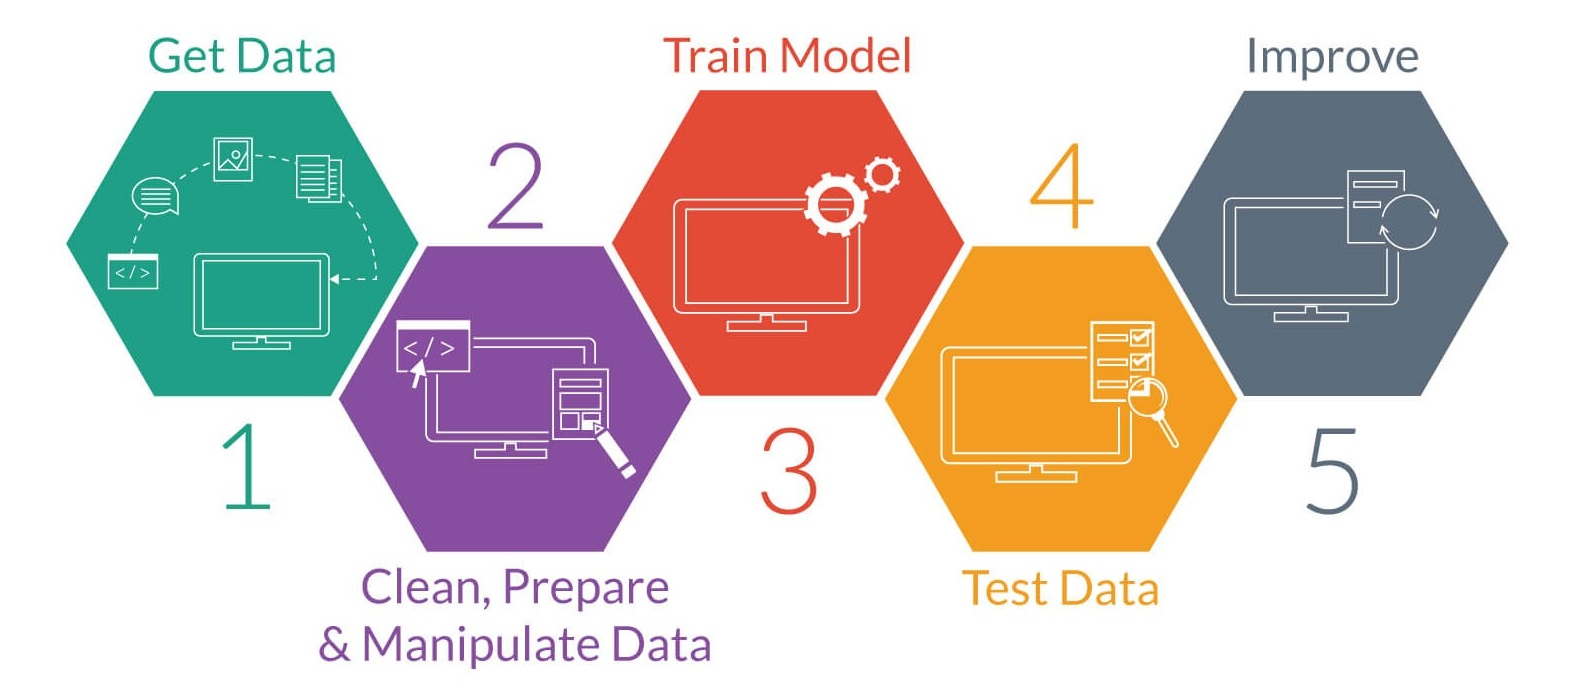
\includegraphics[width=0.8\textwidth]{Figures/machine_learning.jpg}
  \caption{5 steps for a Machine Learning Model} \citep{Poddar:2016:MachineLearning}
  \label{fig:Poddar:2016:MachineLearning}
  \end{center}
\end{figure}

For the training of the \gls{ML} model according to the approach in figure \ref{fig:Poddar:2016:MachineLearning}, the first step of the methods applied, as illustrated in figure \ref{fig:MachineLearningModelComponents}, is to obtain previously-labeled training data from the freely accessible AFEW-VA database \citep{Kossaifi:2017:AFEW-VADatabase}. It consists of naturally created data, extracted from 600 challenging real-world video clips. For each clip, per-frame annotations are provided with 68 facial landmarks, as well as values for valence (how negative or positive the experience is) and arousal (how calming or exciting the experience is).
\newpage

\begin{figure}[H]
  \begin{center}
  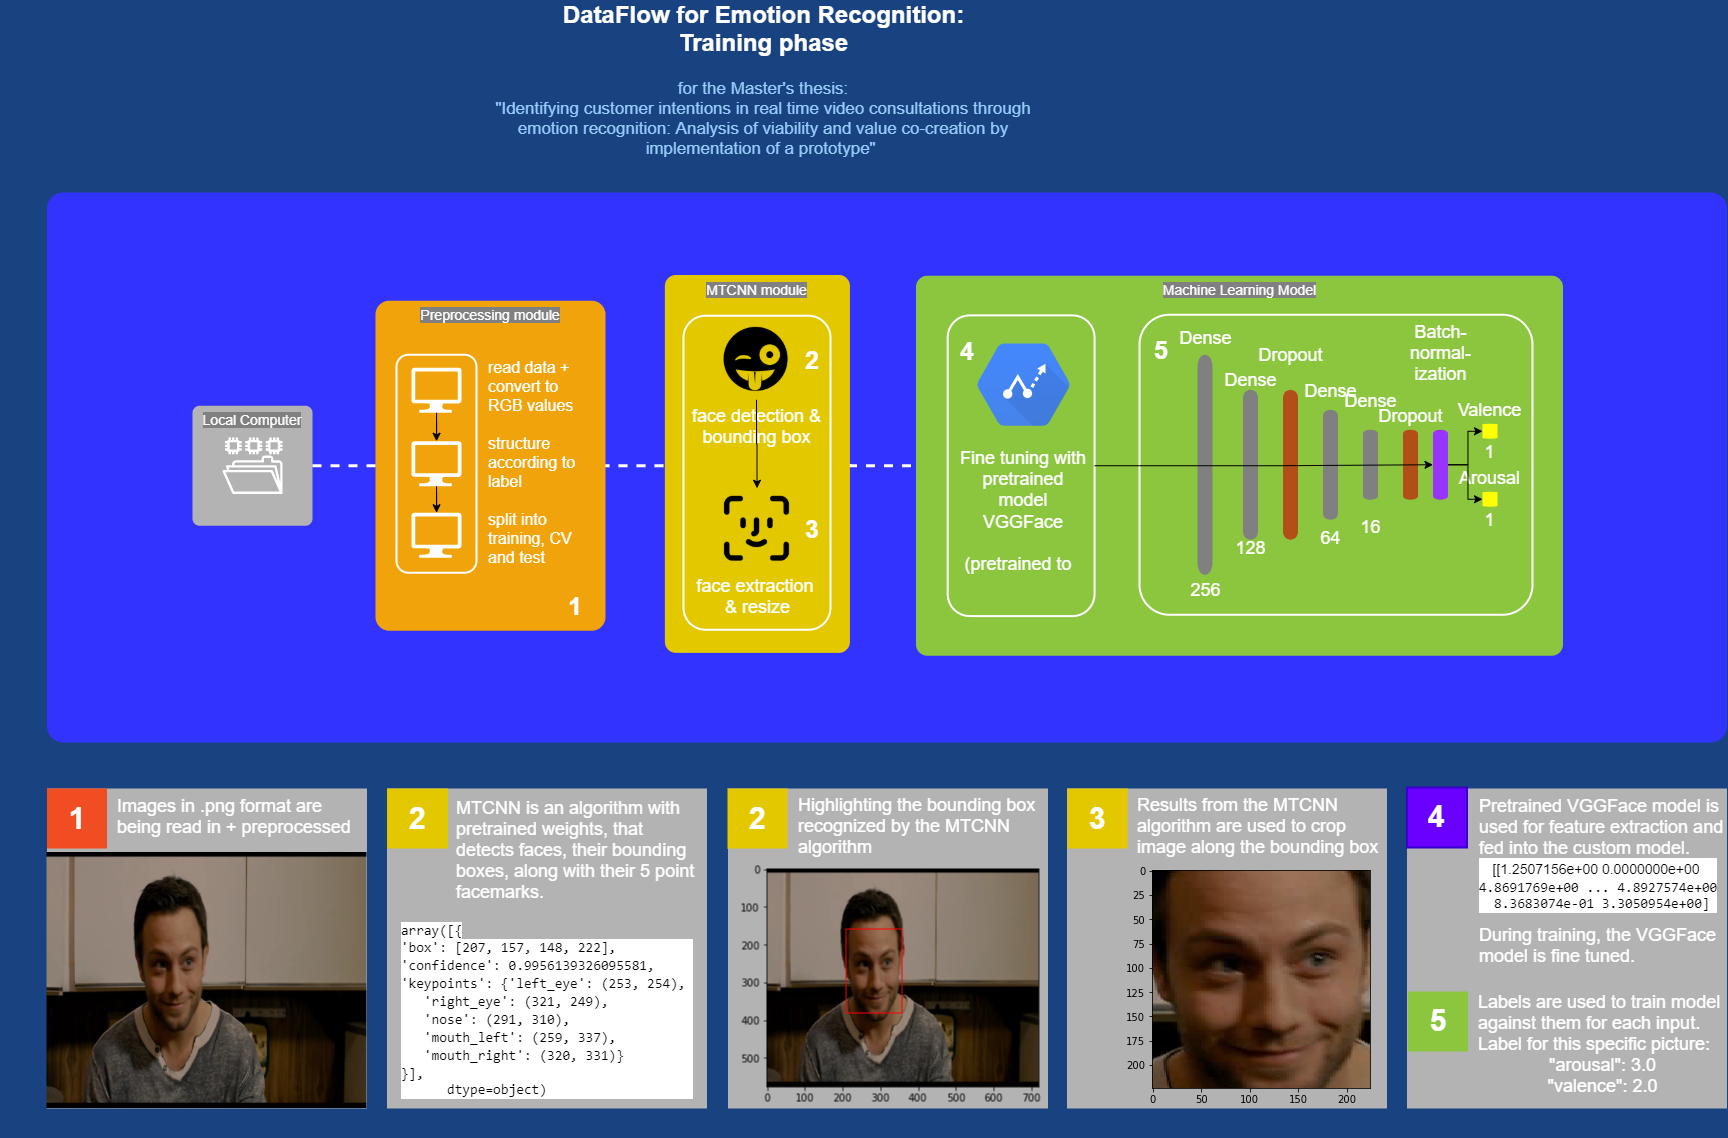
\includegraphics[angle=90, width=0.9\textwidth]{Figures/DataFlow_Diagram_Expose.png}
  \caption{Overview: Machine Learning Model - Components}
  \label{fig:MachineLearningModelComponents}
  \end{center}
\end{figure}

In step \#1, video-frames are converted to RGB values and split into training and validation data. The data might also be restructured depending on the already existing data structure. The result will serve as an input for the model.
\newline\newline
In step \#2, a pretrained network, called \gls{MTCNN} \citep{Zhang:2016:MTCCN} is used to detect human faces and their bounding box in an image. With that data, the image can be cropped according to the detected bounding box in step \#3. At this point, an extra step could be added for further optimization. Thus, making use of the already detected landmarks in step \#2 and reusing them, for example, for constructing an \gls{AAM}. This might allow the model to learn better facial features.
\newline\newline
In the next step, the cropped face is being fed into the Neural Network architecture, which is comprised of a pre-trained network called VGGFace \citep{Cao:2018:VGGFace2} (step \#4) and custom built layers on top (step \#5). The VGGFace network was trained on 3.31 million images and was specifically optimized for face recognition. Therefore, this model should provide very distinct output vectors for the face's features, which will then allow the custom model to learn the mapping between the desired output (= the label) and the given input (= the face's features). This whole architecture, including the VGGFace model, will be further optimized through fine-tuning the whole architecture to better perform on the challenge at hand.

%%%%%%%%%%%%%%%%%%%%%%%%%%%%%%%%%%%%%%%%%%%%%%%%%%%%%%%

\chapter{Results comparison and analysis}
The outcome of the above described methodology will be compared to the following three papers, which will serve as a benchmark:
\begin{itemize}
    \item In the original paper from 2017, when the AFEW-VA database \citep{Kossaifi:2017:AFEW-VADatabase} was introduced, the author already provided a benchmark by comparing different methods, like SVR or DCNN, with the three metrics RMSE (Root Mean Squared Error), CORR (Correlation) and ICC (Interclass Correlation). 
    \item The 'DeepDriver' paper \citep{Theagarajan:2018:DeepDriver} from the year 2018, used the AFEW-VA database to evaluate their approach. Their approach consists of taking multiple frames as a sequence and feeding them into either a CNN-only or a CNN + LSTM architecture. Both methods heavily outperformed all benchmark results on the RMSE and CORR metric.
    \item The authors  \citet{Handrich:2020:SimultaneousPredVA} made use of the AFEW-VA database \citep{Kossaifi:2017:AFEW-VADatabase} for their training on the recognition of valence and arousal in videos/images. Thus, they could achieve slightly better results for the CORR and ICC metrics than the original paper. Furthermore, they improved their own approach through using multiple databases for cross-validation. Their results show, that their results are indeed an improvement to the 2017 benchmark paper, compared to the DeepDriver paper from 2018, however, the results are still lagging behind.
\end{itemize}

As all of these papers use different approaches for their neural network architecture in order to solve this \gls{ER} task, it is indeed valuable to keep different approaches in mind when comparing the results of this Master thesis to the state-of-the-art. Gladly, all three papers make use of the RMSE and CORR metric, which allows me to objectively compare my obtained results with these papers.


%%%%%%%%%%%%%%%%%%%%%%%%%%%%%%%%%%%%%%%%%%%%%%%%%%%%%%%

\chapter{Application of results}
\textbf{Identifying customer intentions}\newline
For the application of \gls{ER} in order to identify human intentions in real-time video calls, a mechanism needs to be developed, which maps the 2-dimensional emotion values (valence and arousal) to a measure of interest. The hypothesis here is, that whenever an emotion was correctly predicted, an intention or level of interest can automatically be deducted. This application will be evaluated with an experiment in order to assess for PPI AG the viability of further pursuing this approach. A possible experiment might be a video call with multiple test persons that are asked to answer controversial statements and are afterwards asked to rate their own interest in each statement. This will be compared with the identified intention/interest through \gls{ER}.
\newline\newline
\textbf{Can the identification of customer intentions facilitate a co-creation of value in real-time video calls?}\newline
Under the hypothesis that it is possible to identify customer intentions, the question here is whether it can be shown that \gls{ER} can deliver value to both consultant and customer. This could be confirmed by showing that such an approach can theoretically be integrated with an application to improve dynamic content generation, e.g. a chat-bot. In a prototypical implementation, the chat-bot behavior could be imitated by a simple decision tree which gets triggered by a defined event and bases its decisions on the current level of interest.

%%%%%%%%%%%%%%%%%%%%%%%%%%%%%%%%%%%%%%%%%%%%%%%%%%%%%%%

\chapter{Timeline}
\begin{comment}
Legen Sie sich einen groben Zeitplan fest, wann Sie welche Phase der Abschlussarbeit beginnen und beenden wollen. Berücksichtigen Sie dabei auch Puffer für Krankheiten, private Veranstaltungen und Korrekturzeiten. Wenn ein Praxispartner involviert ist, beachten Sie auch dessen Termine (wie bspw. Urlaub, Weihnachtszeit).

•	Tabellarische Auflistung
o	Aufgaben mit ggf. Unteraufgaben
o	Der verwendeten Methodik
o	Das Ergebnis
o	Hilfreiche Fragestellungen zur Lösung der Aufgabe
o	Geplanter Zeitraum
\end{comment}

For the construction of a timeline the work is divided into the following phases and tasks:
\begin{enumerate}
    \item Solution Design
    \begin{itemize}
        \item Requirements specification
        \item Creation of a solution concept
        \item Elaboration of a scientific Exposé
    \end{itemize}
    \item Technical Design
    \begin{itemize}
        \item Literature review
        \item Data acquisition \& preparation
        \item ML Model for Facial Emotion Recognition
    \end{itemize}
    \item Iterative Implementation (MVP/Prototype)
    \begin{itemize}
        \item Building
            \begin{itemize}
                \item Training and Analysis of \gls{ER} Model
                \item Application with real-time \gls{ER}
            \end{itemize}
        \item Intervention
            \begin{itemize}
                \item Regular meetings with supervisors
                \item Expert interviews
            \end{itemize}
        \item Evaluation
            \begin{itemize}
                \item \gls{ER} results comparison to benchmark papers
                \item Fulfillment of thesis objectives
            \end{itemize}
    \end{itemize}
    \item Revision
    \begin{itemize}
        \item Organization of documentation 
        \item Finishing the formulation of the thesis
        \item Revision of Master thesis 
    \end{itemize}
\end{enumerate}
\vspace*{1cm}

As all of these items are conducted in an iterative approach, it is assumed that evaluation of tasks will take place immediately before each task was completed. There will be a strong focus on a constant exchange with my supervisor. Therefore, the only fixed dates that can be aimed at in advance for this Master thesis are the registration date, as well as the hand-in date of the final Master's thesis. With this in mind, I plan to register the thesis by the 15th of June 2020 and thus, my time-window of 6 months working time will end on the 15th of December 2020.
\newline\newline
The following illustration clearly displays the phases of this Master thesis together with its major milestones:
\newpage

\begin{landscape}
\begin{center}

\begin{tikzpicture}[timespan={}]% no label is displayed for the timespan
  \timeline[custom interval=true]{May, June, July, August, September, October, November, December}
  \begin{phases}
    \initialphase{involvement degree=4cm,phase color=blue}
    \phase{between week=2 and 3 in 0.2,
      involvement degree=2cm,phase color=red!50!yellow}
    \phase{between week=3 and 7 in 0.5,
      involvement degree=11cm,phase color=green!50!yellow}
    \phase{between week=7 and 8 in 1.1,
      involvement degree=3cm,phase color=red!50!blue}
  \end{phases}
  
  
  \node [xshift=-0.6cm,yshift=1cm,anchor=east,
         font=\bfseries] at (phase-0.180) {Milestones};
  \node [xshift=-0.6cm,yshift=-1cm,anchor=east,
         font=\bfseries] at (phase-0.180) {Phases};


  \addmilestone{at=phase-0.-90,direction=-90:3.0cm, text={Solution Design}, text options={below}}
  \addmilestone{at=phase-0.-90,direction=-90:3.5cm, text={(Problem Definition)}, text options={below}}
  
  \addmilestone{at=phase-1.-95,direction=-90:2.5cm, text={Technical Design}, text options={below}}
    
  \addmilestone{at=phase-2.-90,direction=-90:1.5cm, text={Iterative implementation}, text options={below}}
  \addmilestone{at=phase-2.-90,direction=-90:2.0cm, text={(Building, Intervention and Evaluation)}, text options={below}}
    
  \addmilestone{at=phase-3.-90,direction=-90:2.5cm, text={Revision}, text options={below}}
  \addmilestone{at=phase-3.-90,direction=-90:3.0cm, text={(Formalization of Learning)}, text options={below}}
    
    
    
    %% Packages vs. Milestones
    \addmilestone{at=phase-0.20,direction=90:2.0cm, text={Exposé finalized}, text options={above}}
    
    \addmilestone{at=phase-2.173,direction=90:4.0cm, text={Registration thesis}, text options={above}}
    \addmilestone{at=phase-2.173,direction=90:3.5cm, text={15.06.2020}, text options={above}}

    \addmilestone{at=phase-2.07,direction=90:4.0cm, text={Prototype finished}, text options={above}}
    
    \addmilestone{at=phase-3.27,direction=90:2.5cm, text={Deadline thesis}, text options={above}}
    \addmilestone{at=phase-3.27,direction=90:2.0cm, text={15.12.2020}, text options={above}}
    
\end{tikzpicture}

\vspace*{\fill}
\end{center}
\end{landscape}



%%%%%%%%%%%%%%%%%%%%%%%%%%%%%%%%%%%%%%%%%%%%%%%%%%%%%%%

\chapter{Provisional list of literature}
\begin{comment}
Geben Sie die wesentlichen Quellen (10+) an und beziehen Sie sich in ihren Ausführungen darauf.
\end{comment}

%Zum Einbinden des BibTeX Files:
\bibliography{literature.bib}{\nocite{*}}



% \appendix
% \addtocontents{toc}{\protect\contentsline{chapter}{Appendix}{}}

% \chapter{Action Design Research (ADR)}

% \begin{figure}[!ht]
%   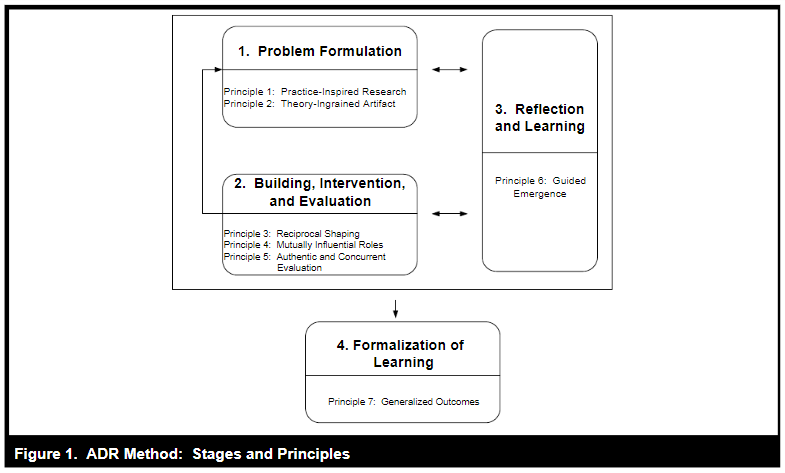
\includegraphics[width=\linewidth]{Figures/Paper_2011_ActionDesignResearch_Method.PNG}
%   \caption{Action Design Research: Method}
%   \label{fig:Sein:2011:ADR:Method}
% \end{figure}

% \begin{figure}[!ht]
%   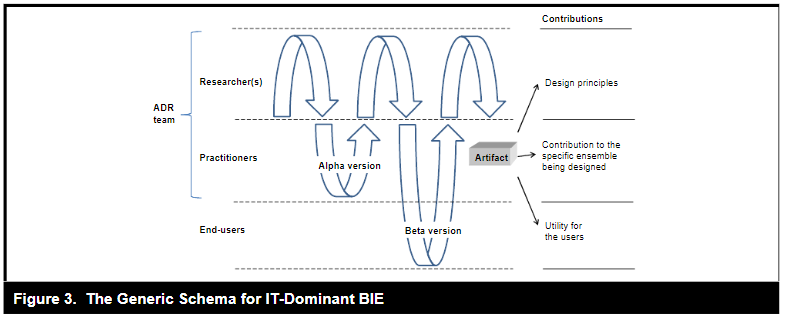
\includegraphics[width=\linewidth]{Figures/Paper_2011_ActionDesignResearch_BIE.PNG}
%   \caption{Action Design Research: Build-Intervention-Evaluation (BIE)}
%   \label{fig:Sein:2011:ADR:BIE}
% \end{figure}





\backmatter

\thispagestyle{empty}

\vspace*{\fill}
\pagestyle{empty}

{\normalsize
\begin{center}\textbf{Sworn declaration}\end{center}
I hereby affirm in lieu of oath that I have independently written the present exposé in the Master's program IT Management and Consulting and that I have not used any tools other than those indicated -- especially no Internet sources not mentioned in the list of sources. All passages that have been taken literally or analogously from publications are marked as such. I further affirm that I have not previously submitted the paper in any other examination procedure.
\vspace*{1cm}\\
Hamburg, \today
\hspace*{\fill}\begin{tabular}{@{}l@{}}\hline
\makebox[5cm]{Tobias Kick}
\end{tabular}

%\vspace*{3cm}
%TODO Dies ist optional, ggf. löschen!
%\begin{center}\textbf{Publication}\end{center}
%I agree to the placement of the work in the library of the Department of Computer Science.
%\vspace*{1cm}\\
%Hamburg, \today
%\hspace*{\fill}\begin{tabular}{@{}l@{}}\hline
%\makebox[5cm]{Tobias Kick}
%\end{tabular}

}
\vspace*{\fill}


\end{document}
